\input{../YKY-preamble.tex}
\setmainfont[BoldFont=AlibabaSans-Regular.otf]{AlibabaSans-Light.otf}

\usepackage[active,tightpage]{preview}		% for continuous page(s)
\renewcommand{\PreviewBorder}{0.5cm}
\renewcommand{\thempfootnote}{\arabic{mpfootnote}}

\usepackage[absolute,overlay]{textpos}		% for page number on upper left corner

\usepackage{color}
\usepackage{mathtools}
\usepackage[hyperfootnotes=false]{hyperref}

% \usepackage[backend=biber,style=numeric]{biblatex}
% \bibliography{../AGI-book}
% \renewcommand*{\bibfont}{\footnotesize}

\usepackage{graphicx} % Allows including images
\usetikzlibrary{shapes}
\usepackage[export]{adjustbox}				% ??
\usepackage{bm}
\usepackage{verbatim} % for comments
% \usepackage[most]{tcolorbox}
% \usepackage{newtxtext,newtxmath}	% Times New Roman font

% \numberwithin{equation}{subsection}

\newcommand{\underdash}[1]{%
	\tikz[baseline=(toUnderline.base)]{
		\node[inner sep=1pt,outer sep=10pt] (toUnderline) {#1};
		\draw[dashed] ([yshift=-0pt]toUnderline.south west) -- ([yshift=-0pt]toUnderline.south east);
	}%
}%

% Tic-Tac-Toe symbols
% \newcommand{\bO}[0]{\raisebox{-0.2em}{\textbf{O}}}
% \newcommand{\Xb}[0]{\raisebox{-0.2em}{\textbf{X}}}

%\DeclareSymbolFont{symbolsC}{U}{txsyc}{m}{n}
%\DeclareMathSymbol{\strictif}{\mathrel}{symbolsC}{74}
\DeclareSymbolFont{AMSb}{U}{msb}{m}{n}
\DeclareSymbolFontAlphabet{\mathbb}{AMSb}
% \setmathfont{Latin Modern Math}

% \newcommand{\highlight}[1]{\colorbox{pink}{$\displaystyle #1$}}

% \newcommand{\emp}[1]{{\color{violet}\textbf{#1}}}
\let\oldtextbf\textbf
\renewcommand{\textbf}[1]{\textcolor{blue}{\oldtextbf{#1}}}

\newcommand*\confoundFace{$\vcenter{\hbox{\includegraphics[scale=0.2]{../2020/../confounded-face.jpg}}}$}
\newcommand{\underconst}{\includegraphics[scale=0.5]{../2020/UnderConst.png}}
\newcommand{\KBsymbol}{\vcenter{\hbox{\includegraphics[scale=1]{../KB-symbol.png}}}}
\newcommand{\witness}{\scalebox{0.6}{$\blacksquare$}}
% \newcommand{\Heytingarrow}{\mathrel{-}\mathrel{\triangleright}}
% \providecommand\Heytingarrow{\relbar\joinrel\mathrel{\vcenter{\hbox{\scalebox{0.75}{$\rhd$}}}}}

\begin{document}

\begin{preview}

\cc{
\title{\vspace{-2.2cm} \bfseries\color{blue}{\large 逻辑化 AGI 基础}}
}{
\title{\vspace{-2.2cm} \bfseries\color{blue}{\large Logical AGI basic framework}}
}

% \author{YKY} % Your name
\date{\vspace{-3.2cm}} % Date, can be changed to a custom date

\maketitle

\setcounter{section}{-1}

% (1) Circled page number on upper left corner
\begin{textblock*}{5cm}(2.1cm,2.3cm) % {block width} (coords) 
{\color{red}{\large \textcircled{\small 1}}}
\end{textblock*}

\begin{minipage}{\textwidth}
\setlength{\parskip}{0.4\baselineskip}

\cc{
这是 \textbf{强化学习} 最基本的 setup}{
This is our basic \textbf{RL} (reinforcement learning) setup}\footnote{The above diagram is somewhat inaccurate as there are subtle differences between the notions of "state" and Working Memory.  In RL, state usually refers to the external environment  through observations.  WM is slightly different in the sense that an internal belief may be \textit{wrong} about the environment --- eg, mistaking seeing something that doesn't exist.  There is on-going research as to the relation between RL and WM.  I have not fully resolved this issue.
	\begin{equation}
	\vcenter{\hbox{\includegraphics[scale=0.5]{../2021/RL-WM-architecture.png}}}
	\end{equation}
	\vspace{-0.7cm}}:
\begin{equation}
\vcenter{\hbox{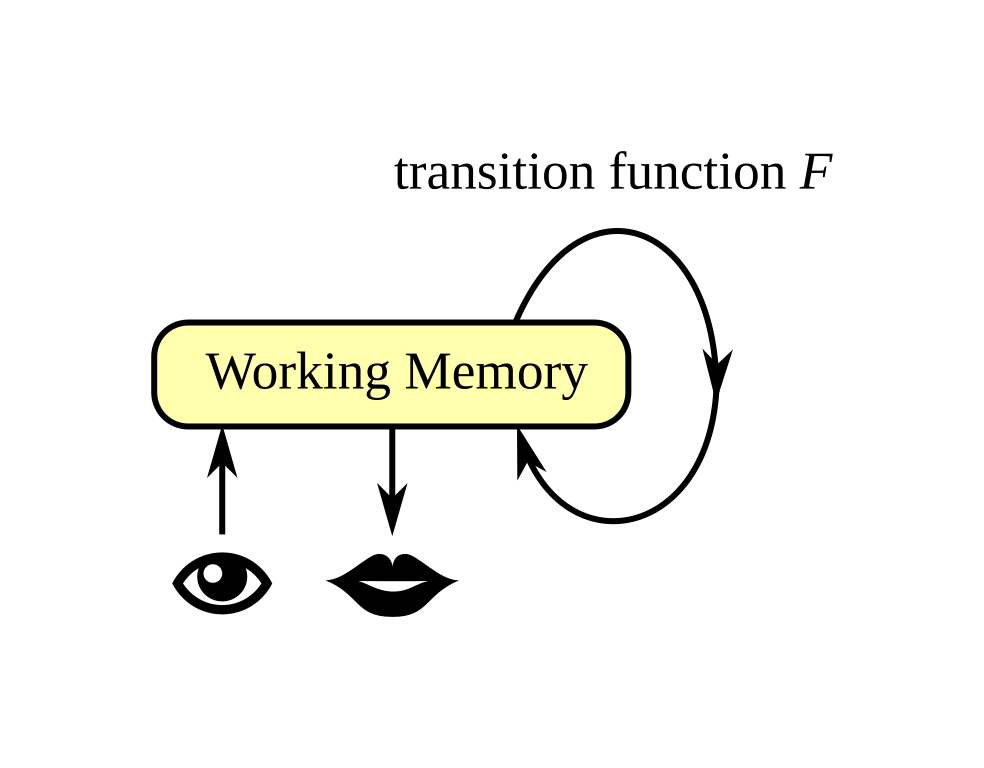
\includegraphics[scale=0.7]{../2021/minimal-RL-architecture.png}}}
\end{equation}
\cc{
	状态转移函数 $F$ 负责 \textbf{更新} 工作记忆 (\textbf{WM}). 如果 $F$ 在一个 \textbf{闭环} 内训练,它似乎可以 ``\textbf{解释}'' (或 预测) 输入的讯息。
}{
\textbf{WM} (working memory) is \textbf{updated} by a transition function.  If this transition function is trained in a \textbf{closed loop}, it may be able to "explain" (in the sense of predicting) the input data.	
}

In classical logic-based AI, \textbf{inductive learning} means searching for a \textbf{theory} $T$ (= set of logic rules) that "explains" or \textbf{implies} positive examples but not negative ones:
\begin{equation}
\mbox{\large\(
T \vdash e^{+}, \quad T \nvdash e^{-}
\)}
\end{equation}
While logic learning is powerful, it relies on \textbf{combinatorial search} and was too inefficient, which caused "AI Winter".

I want to argue that the function $F$ can be trained to perform like the set of logic rules $T$.  
\end{minipage}
\end{preview}

\begin{preview}
\setlength{\parskip}{0.4\baselineskip}
% (2) Circled page number on upper left corner
\begin{textblock*}{20cm}(2.1cm,2.3cm) % {block width} (coords) 
	{\color{red}{\large \textcircled{\small 2}}}
	\hspace{7cm}
	\bfseries\color{blue}{\small 逻辑化 AGI 基础}
\end{textblock*}

\vspace*{0.7cm} The ``standard model'' is a way of thinking, that may help us better understand the general theory of AGI systems.

The essence of the standard model is just to identify a \textbf{Working Memory} as the ``state'' of the AGI system.

One benefit of our theory is that it relates Transformers / BERT / GPT to AGI systems.  These language models are phenomenally intelligent, yet many people criticize them as not ``truly'' intelligent.  The standard model suggests that they are indeed linked to AGI.

\section{Reinforcement learning}

This is the simplest form of a \textbf{dynamical system}:
\begin{equation}
\begin{tikzpicture}[->]
\node[rectangle,draw,label=0:{{$\quad =$} ``working memory"}] (C) {state $x$};
\path (C) edge [out=30,in=150,looseness=4,thick] node [above] {transition function $F$} (C);
\end{tikzpicture}
\end{equation}
When we add a ``control'' or ``action'' variable $a$ to it, it becomes the most basic  \textbf{control system}:
\begin{equation}
\begin{tikzpicture}[->]
\node[rectangle,draw] (C) {$x$};
\path (C) edge [out=30,in=150,looseness=7,thick] node [above] {$F(x, a)$} (C);
\end{tikzpicture}
\end{equation}
which is the setting for Dynamic Programming or \textbf{Reinforcement Learning}.  The optimal solution for such systems is governed by the \textbf{Hamilton-Jacobi-Bellman equation} \footnote{The Hamilton-Jacobi differential version turns out to be not very fruitful from the computational point of view, as far as I know.}:
\begin{equation}
V^*_t = \max_a \mathbb{E} [ R_{t+1} + V^*_{t+1} ]
\end{equation}

TO-DO:  It would be worthwhile to find the brain mechanism that approximates reinforcement learning and use it to help the design of AGI.  

Recently, Yann LeCun's \textbf{Energy-Based Models} offers a way to circumvent the problem of learning probability distributions over actions, when the action space is hugely high-dimensional.  This seems to be an important step towards AGI systems.

I call this the ``standard model'' because of the extreme simplicity of this setup, and that I don't know of other alternative models that deviate much from it.

%\section{The standard model in relation to other systems}

The following diagram shows how the standard model relates to several other important areas, so we can reap profits from their interactions:

\begin{equation}
\vcenter{\hbox{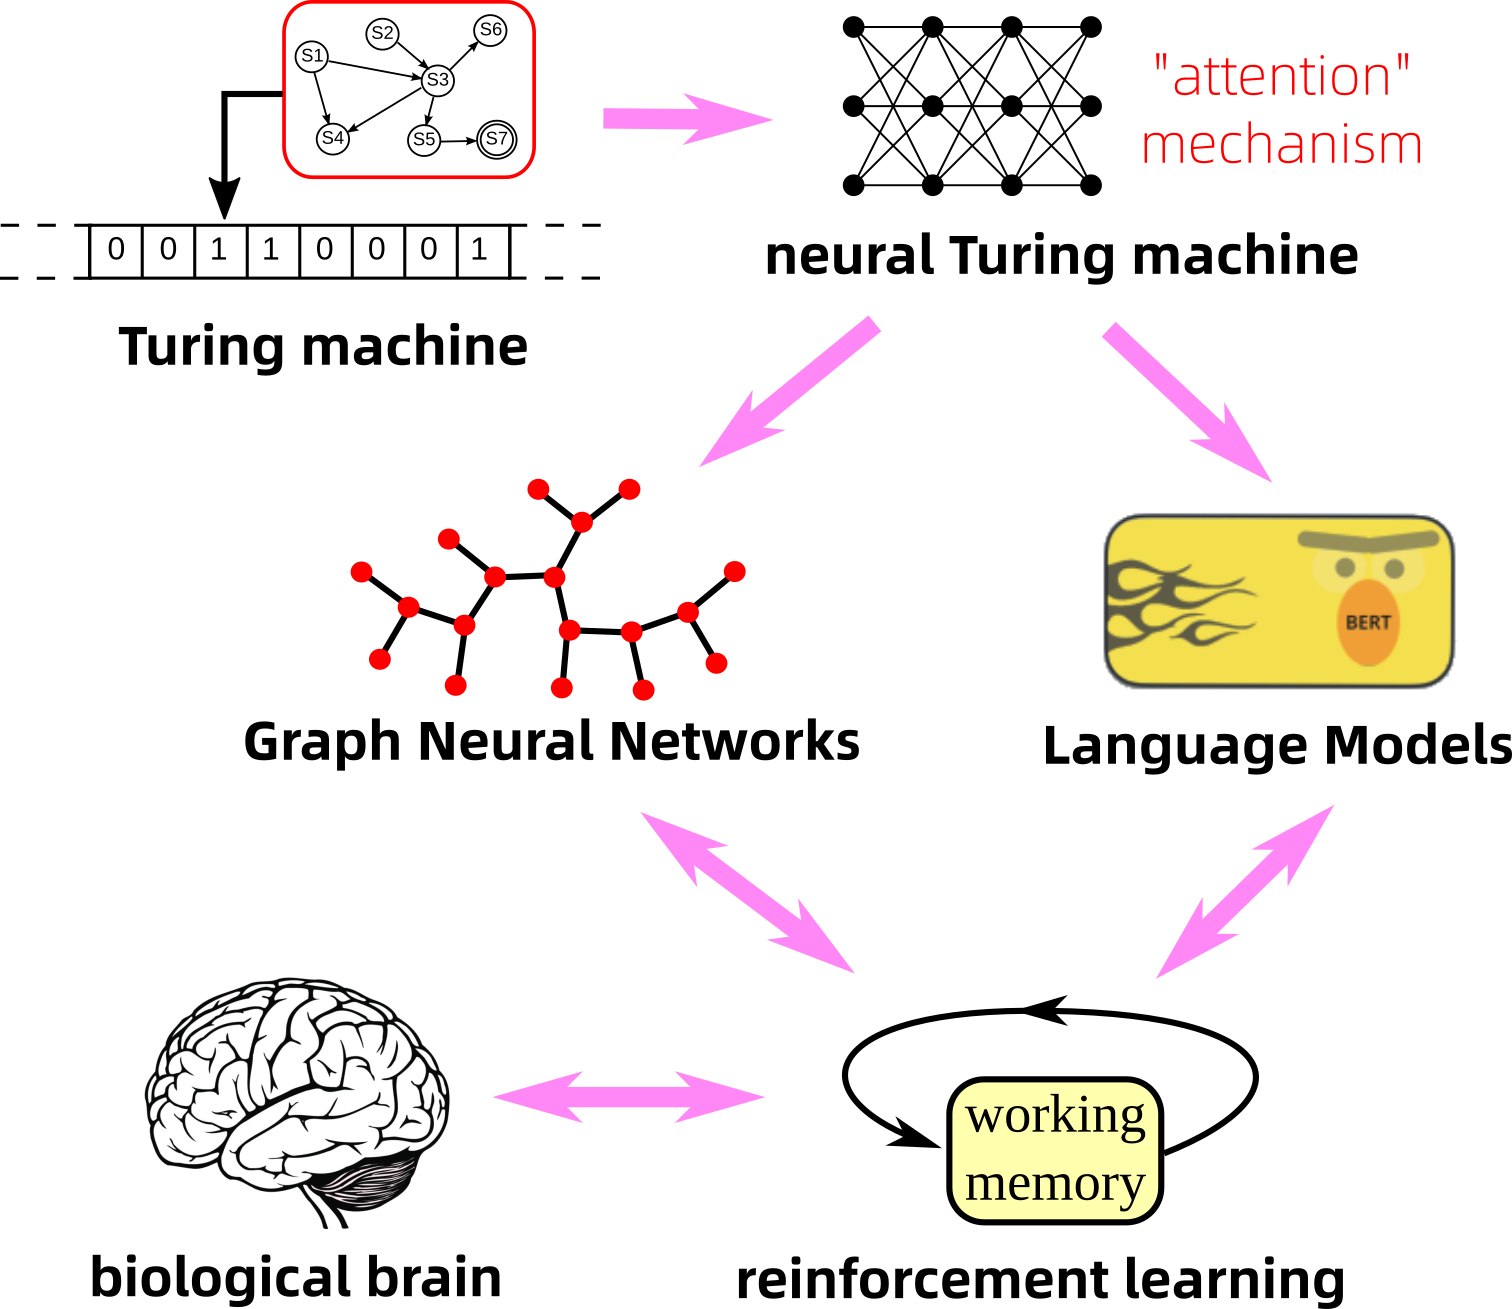
\includegraphics[scale=0.8]{AGI-standard-model.png}}}
\end{equation}

\section{Neural Turing Machines and Transformers}

The \textbf{attention mechanism} was first proposed in the ``\textbf{Neural Turing Machine}''  paper by Graves \textit{et al} [2014].

Recall that a Turing machine is a \textbf{Finite State Machine} augmented with a \textbf{Memory Tape}:
\begin{equation}
\vcenter{\hbox{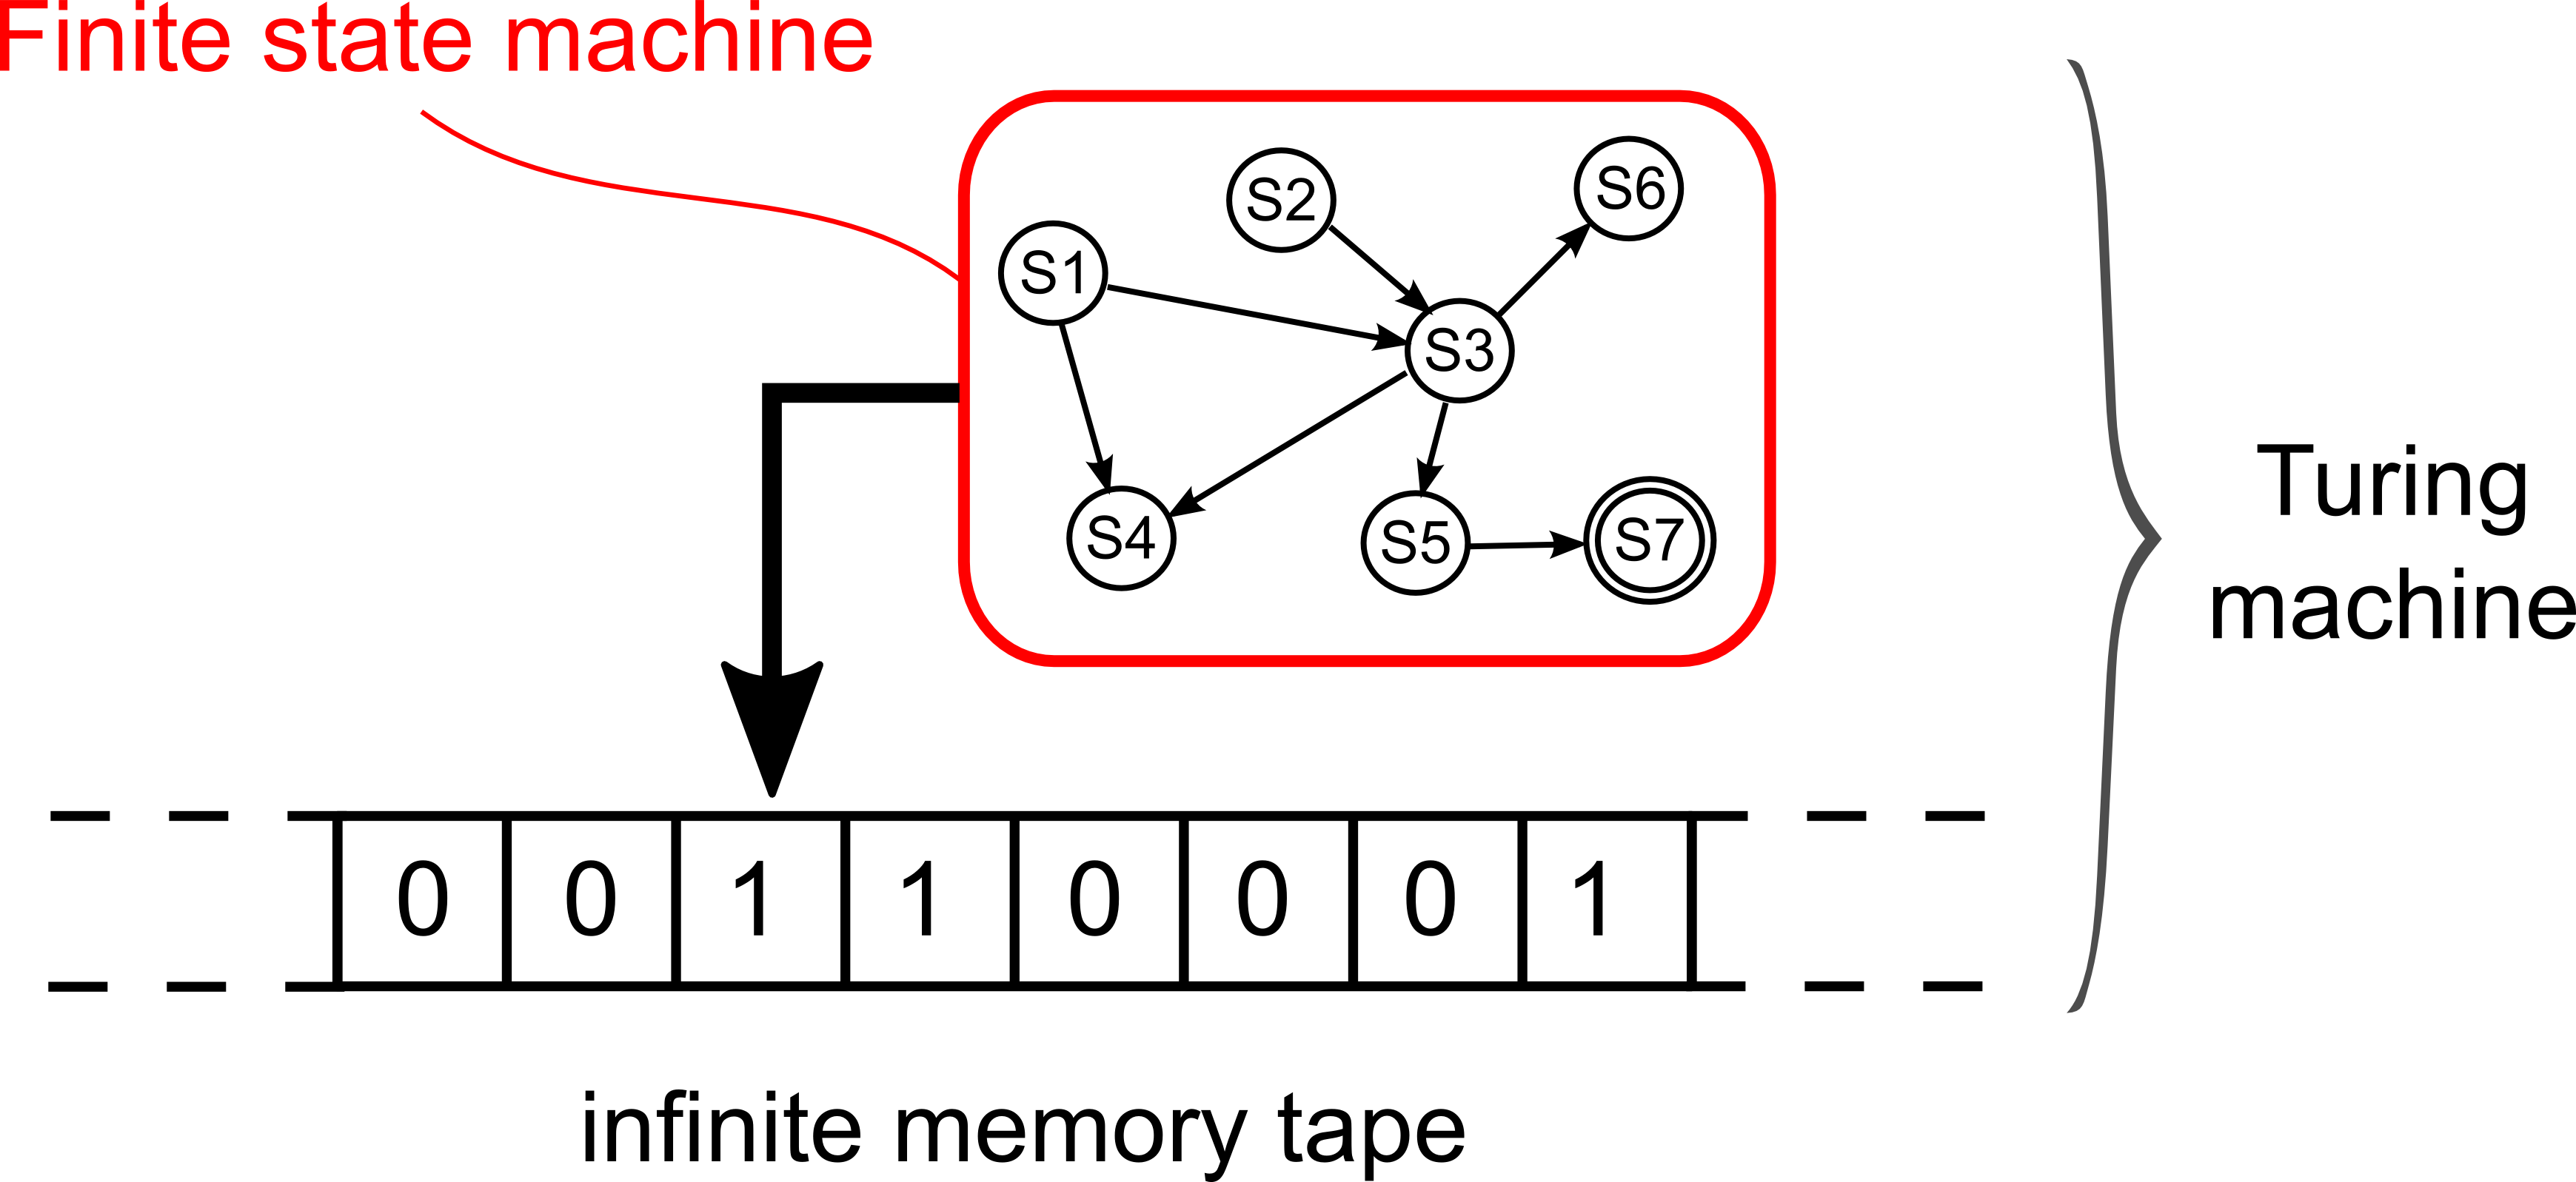
\includegraphics[scale=0.9]{Turing-machine.png}}}
\end{equation}

In Neural Turing Machines, Graves \textit{et al} proposed the attention mechanism for an RNN ``Controller'' (playing the role of the Finite State Machine) to read and write from a \textbf{Memory Matrix} (the tape), using a content-based addressing method.

The Memory Matrix $M$ consists of $N$ items, each of constant size.  \textit{The discreteness of the address would introduce discontinuities in gradients of the output}, hence we need an \textbf{Attention Vector} to focus on a specific location in the memory matrix $M$.

The Attention Vector $\vec{a}$ is calculated via the following formula, familiar to students of the Transformer: 
\begin{equation}
\vec{a} = \mathrm{soft} \max_i \{  \mathcal{D}(K, M_i) \}
\end{equation}
where $D()$ is a similarity measure between the key $K$ and memory item $M_i$.  The key $K$ is emitted by the Controller as the value that it is looking for.

This then evolved into the \textbf{Self Attention} mechanism used in all Transformers.  Now let us refresh with this diagram illustrating Self-Attention (redrawn from a blog article on the web):

\begin{equation}
\vcenter{\hbox{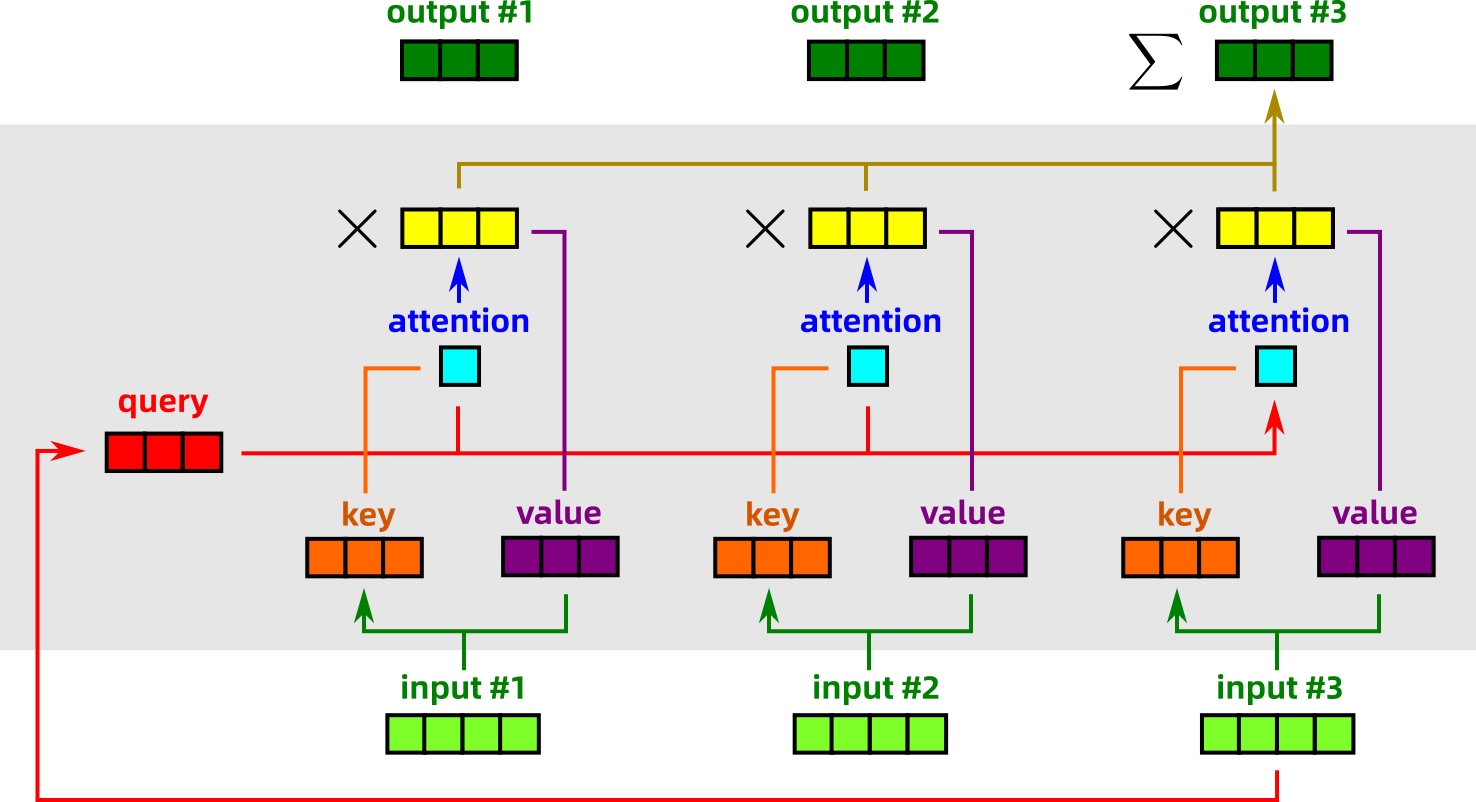
\includegraphics[scale=0.9]{self-attention-2.png}}}
\end{equation}

The research done by Olah \textit{et al}, in their 2021 paper \textit{\uline{A Mathematical Framework for Transformer Circuits}}, is very helpful towards understanding Transformers and Self-Attention.  

For example when we say ``all men are mortal'':
\begin{equation}
\forall x. \; \mbox{Human}(x) \Rightarrow \mbox{Mortal}(x)
\end{equation}
any object instantiated as $x$ (eg. ``Socrates'') would have to be \textbf{copied} from the LHS to the RHS.

\section{Relation to the biological brain}

There are two distinct aspects in the brain:
\begin{itemize}
	\item \textbf{Short-term} or Working Memory is the \textbf{electric activation} of neuronal populations.
	\item \textbf{Long-term} memory is stored as \textbf{synaptic strengths}, established by synaptic formation and strengthening.  The transfer from STM to LTM is called \textbf{memory consolidation}.
\end{itemize}

One theory has it that the prefrontal cortex maintains a number of ``thoughts'' with sub-populations or, perhaps, with \textbf{micro-columns}.  These activated sub-populations are in competition with each other, through \textbf{lateral inhibition}.  The thought(s) that win are the thoughts we retain -- they ``make sense''.

\subsection{How does symbolic logic emerge in the brain?}

\subsubsection{Disentangled features}

If a room of people see a cat enter the room, one person will say ``There's a cat in the room!'' but afterwards it would be \textbf{redundant} for others to say exactly the same thing.  Likewise, in a neural network, if two output features both identify ``cat'' then they are redundant, a waste of resources.  So it is more efficient for one feature vector to move away to a new location in \textbf{feature space}:
\begin{equation}
\vcenter{\hbox{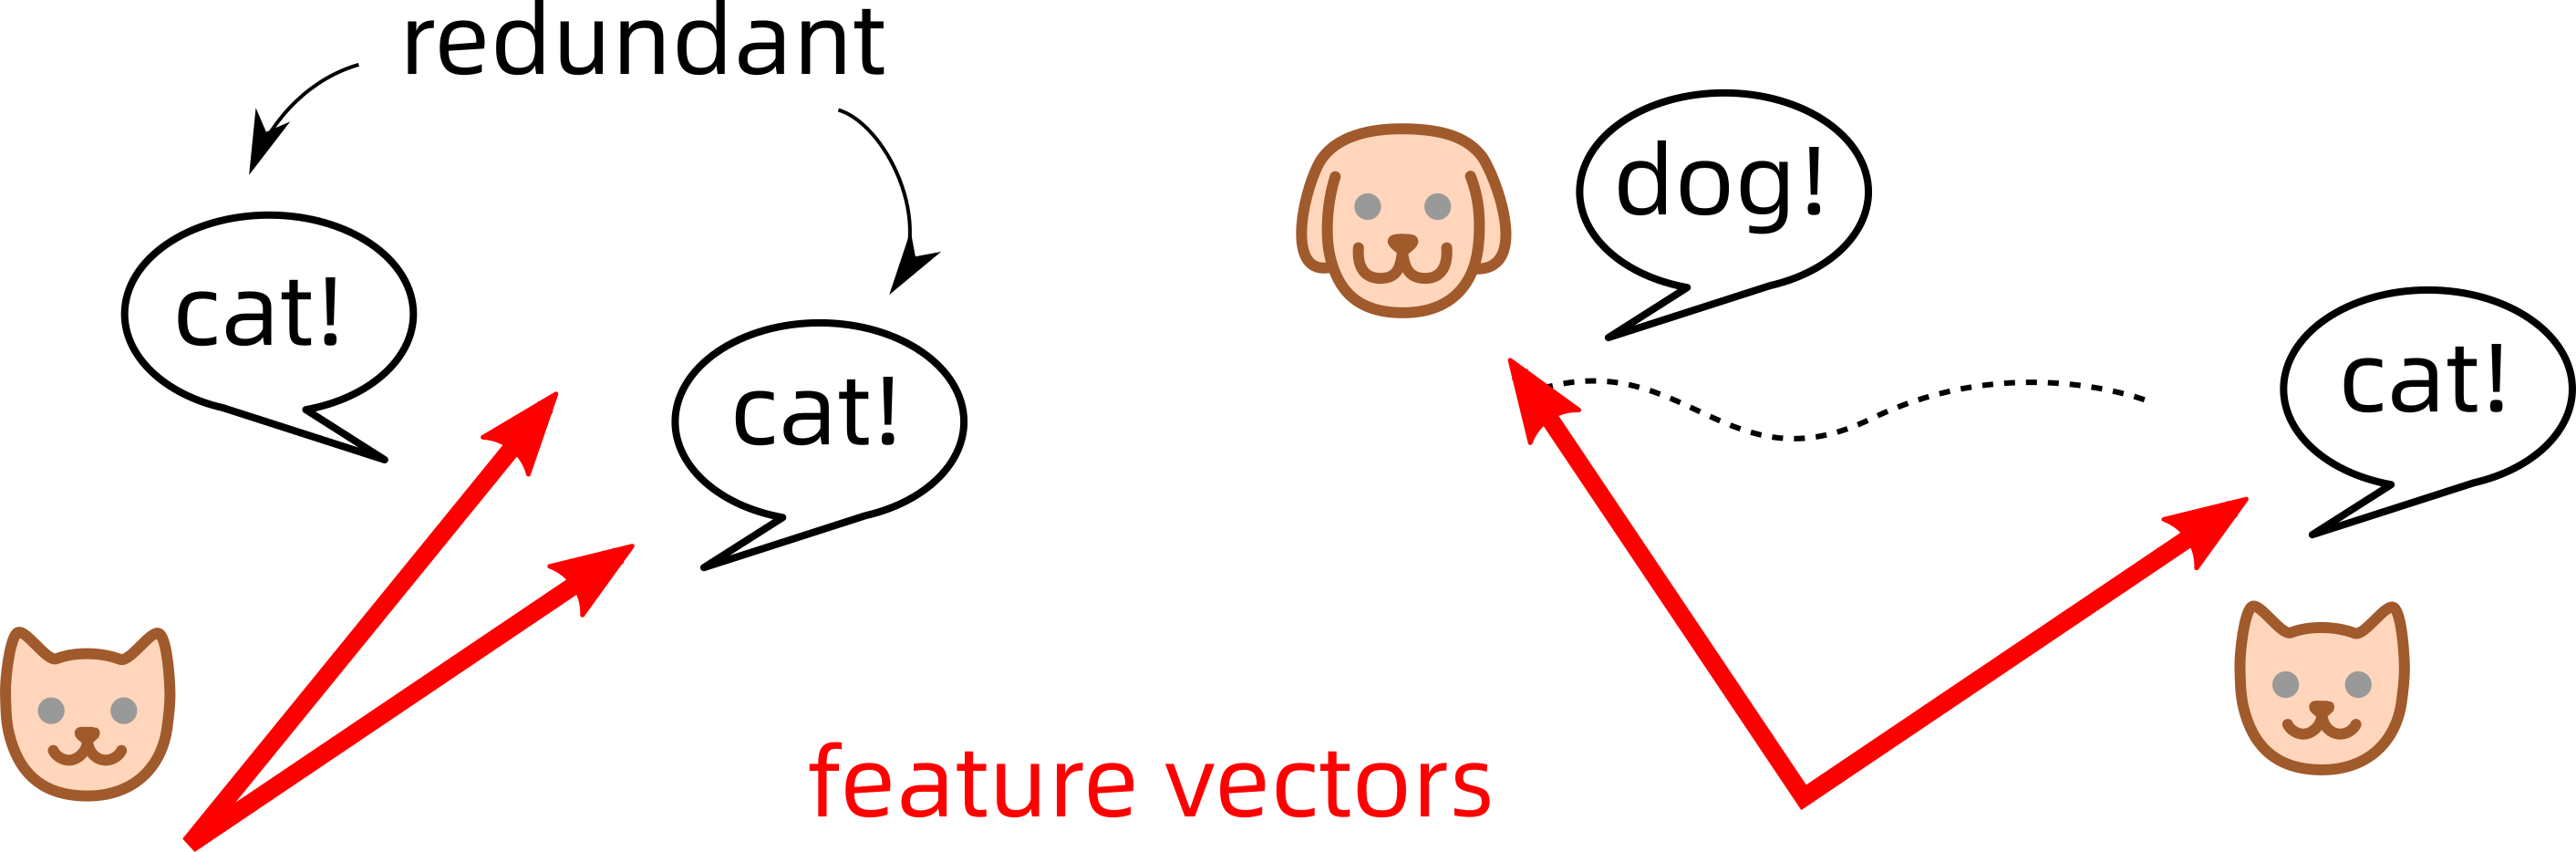
\includegraphics[scale=0.7]{disentangled-features.png}}}
\end{equation}
The result is the emergence of \textbf{disentangled features}.  There is now a lot of research papers on this topic;  Personally I first learned of this from Marta Garnelo and Murray Shanahan's paper  Shanahan2019.  We can think of this as a first step of \textbf{symbolization}, in which objects are recognized by symbols.

In the cortex, neuronal populations are organized into ``columns'', with \textbf{lateral inhibition}  among themselves.  When one population is activated, it suppresses the activation of nearby populations.  This is likely to be the mechanism that enables disentangled features to emerge:
\begin{equation}
\vcenter{\hbox{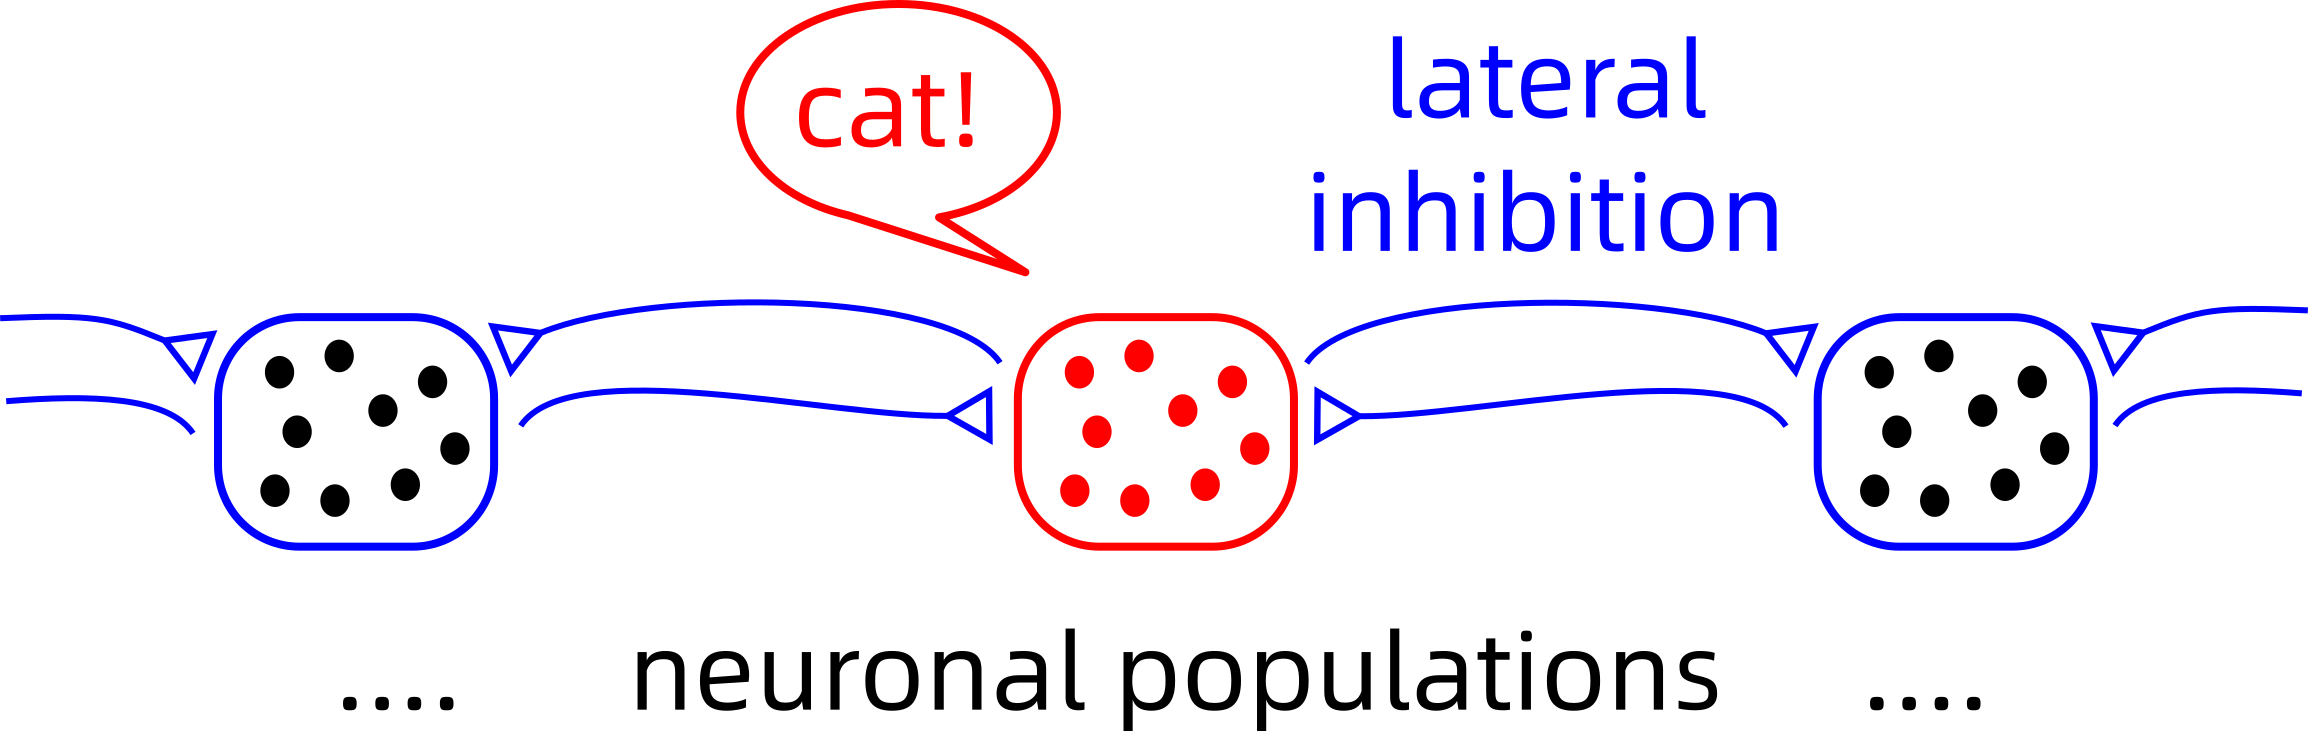
\includegraphics[scale=0.7]{lateral-inhibition.png}}}
\end{equation}
It is remarkable that the \textbf{softmax} in the Transformer / Self-Attention seems to be an abstract implementation of this winner-takes-all \textbf{selection} mechanism.

\subsubsection{Bi-directional connections in the cortex}

Moreover, the cortex is organized into \textbf{layers} with widespread recurrent (ie, forward and backward) connections \footnote{More accurately, there exist two distinct structures: the cortex has a 6-layer structure which has recurrent connections within it;  and each cortical area has bi-directional connections to and from other areas (which may have hierarchical relations among themselves).  I have sort of glossed over this level of details.}:
\begin{equation}
\vcenter{\hbox{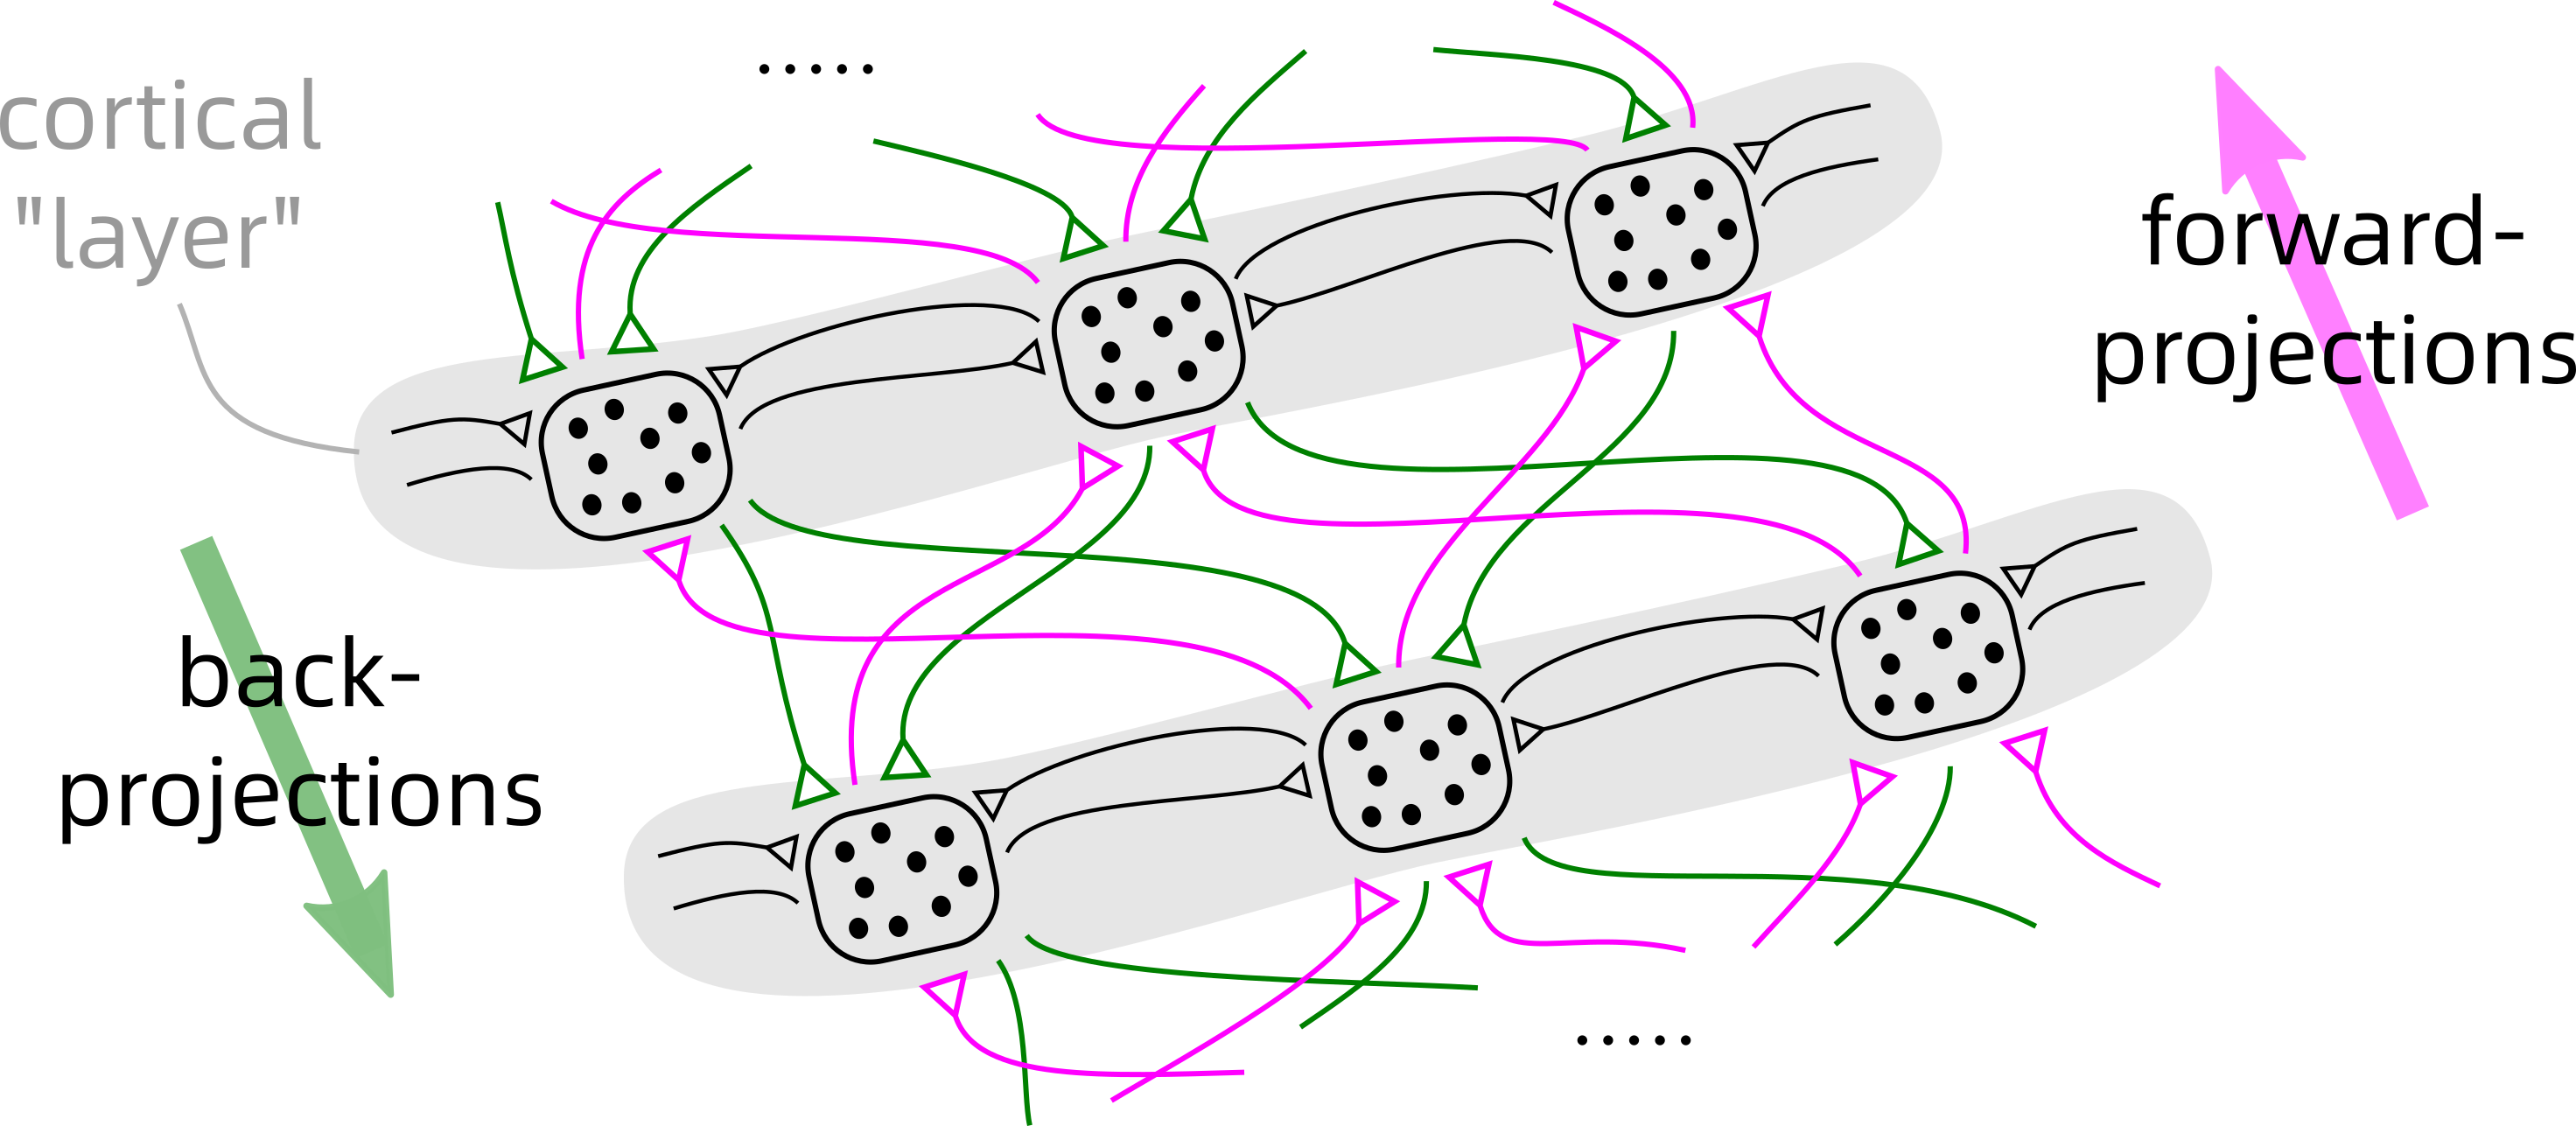
\includegraphics[scale=0.7]{cortex-back-projections.png}}}
\label{fig:cortex-back-projections}
\end{equation}
This bi-directional architecture may be applicable to AGI architecture (see also \S\ref{sec:abductive-reasoning} on abductive reasoning), possibly replacing the current uni-directional model of feed-forward networks and the back-propagation algorithm.

\subsubsection{Alternative to back-propagation?}

As is well-known, the brain does not use back-prop.  The bi-directional innervation is a very significant brain architectural feature that has not yet been incorporated into current deep learning techniques.

In order to find an alternative to back-prop, we need to ask:  What is the essence of deep learning?  I think the answer lies in two words, ``hierarchical'' and ``learned''.  As a counter example, decision trees are hierarchical structures that are learned, but the learning algorithm is too slow because it uses combinatorial search (reminiscent of NP hardness).

But the brain must have a roughly equally powerful learning mechanism as back-prop.  A likely candidate is \textbf{resonance}.  In figure (\ref{fig:cortex-back-projections}) we have a hierarchically connected cortical structure.  What we need is some sort of ``infinitesimal'' learning rule.

\subsubsection{Hierarchy of features}

If we consider relations between objects, for example, ``spoon inside a glass'', this too can emerge out of disentanglement of features, because it is a very \textbf{economical} / efficient representation of a complex scene:
\begin{equation}
\vcenter{\hbox{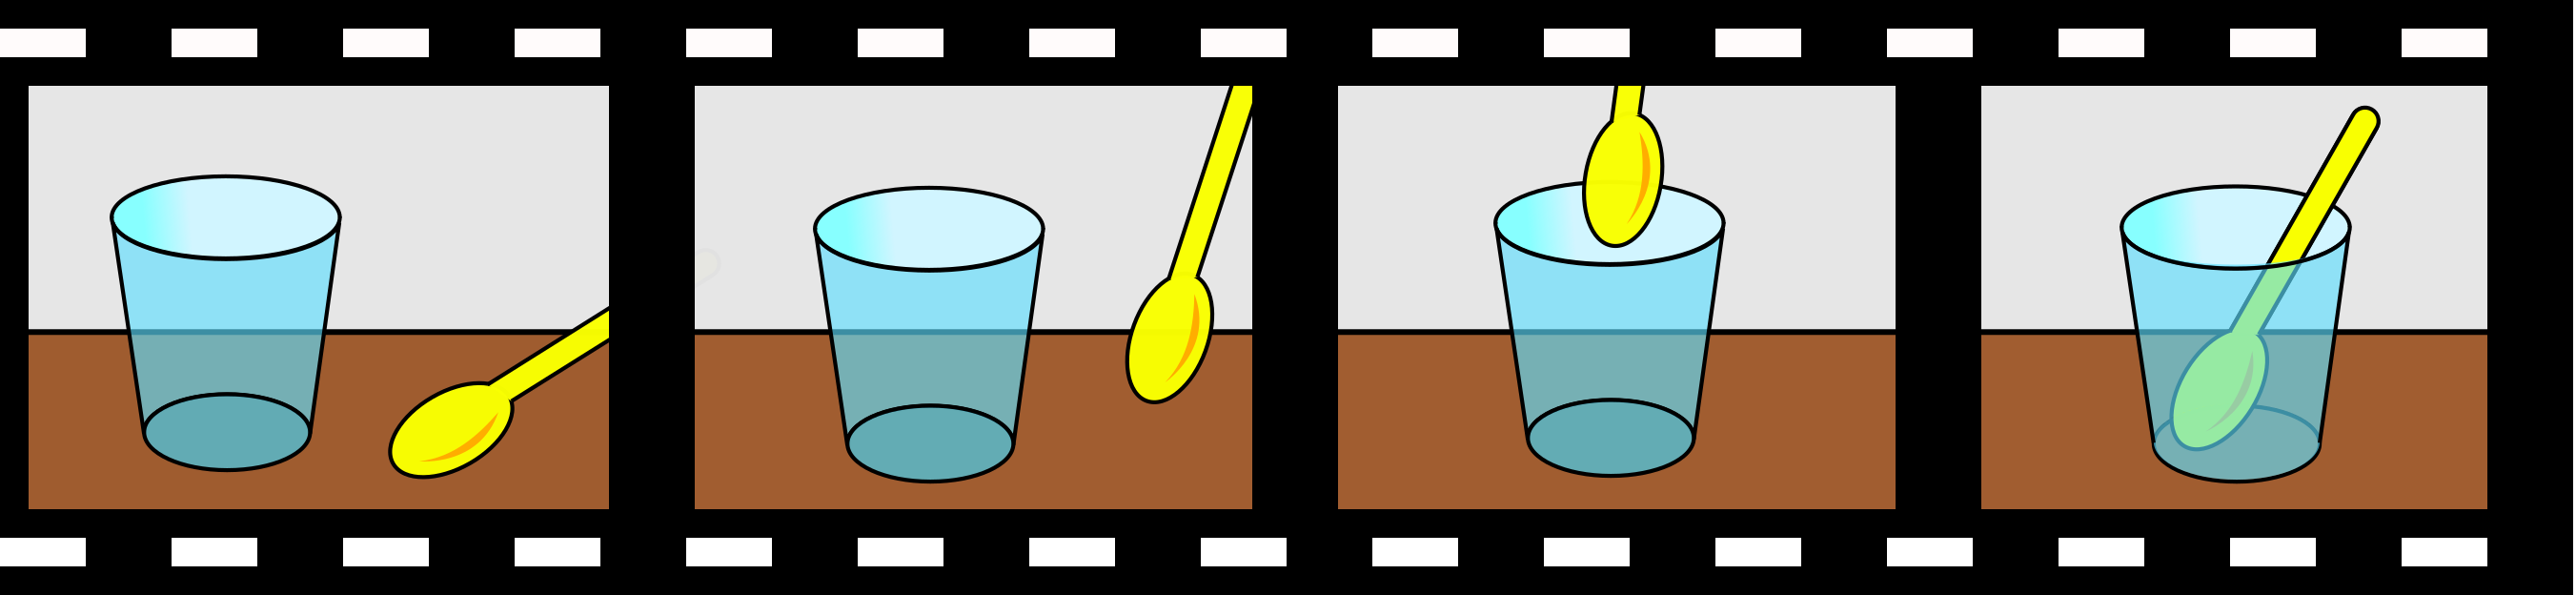
\includegraphics[scale=1]{spoon-in-glass-movie.png}}}
\end{equation}
Every human can recognize this as ``putting a spoon into a glass'', a symbolic representation.  Many researchers may have under-estimated how much the brain uses symbolic reasoning, and my proposal is that AGI can be based entirely on it.  

One remaining question is how to represent symbolic data in a ``neural'' manner.  A general form of symbolic data may be as a \textbf{tree}.  Taking inspiration from the cortex (\ref{fig:cortex-back-projections}), we may perhaps represent the tree / symbolic data as hierarchically organized neural \textbf{feature vectors}:
\begin{equation}
\vcenter{\hbox{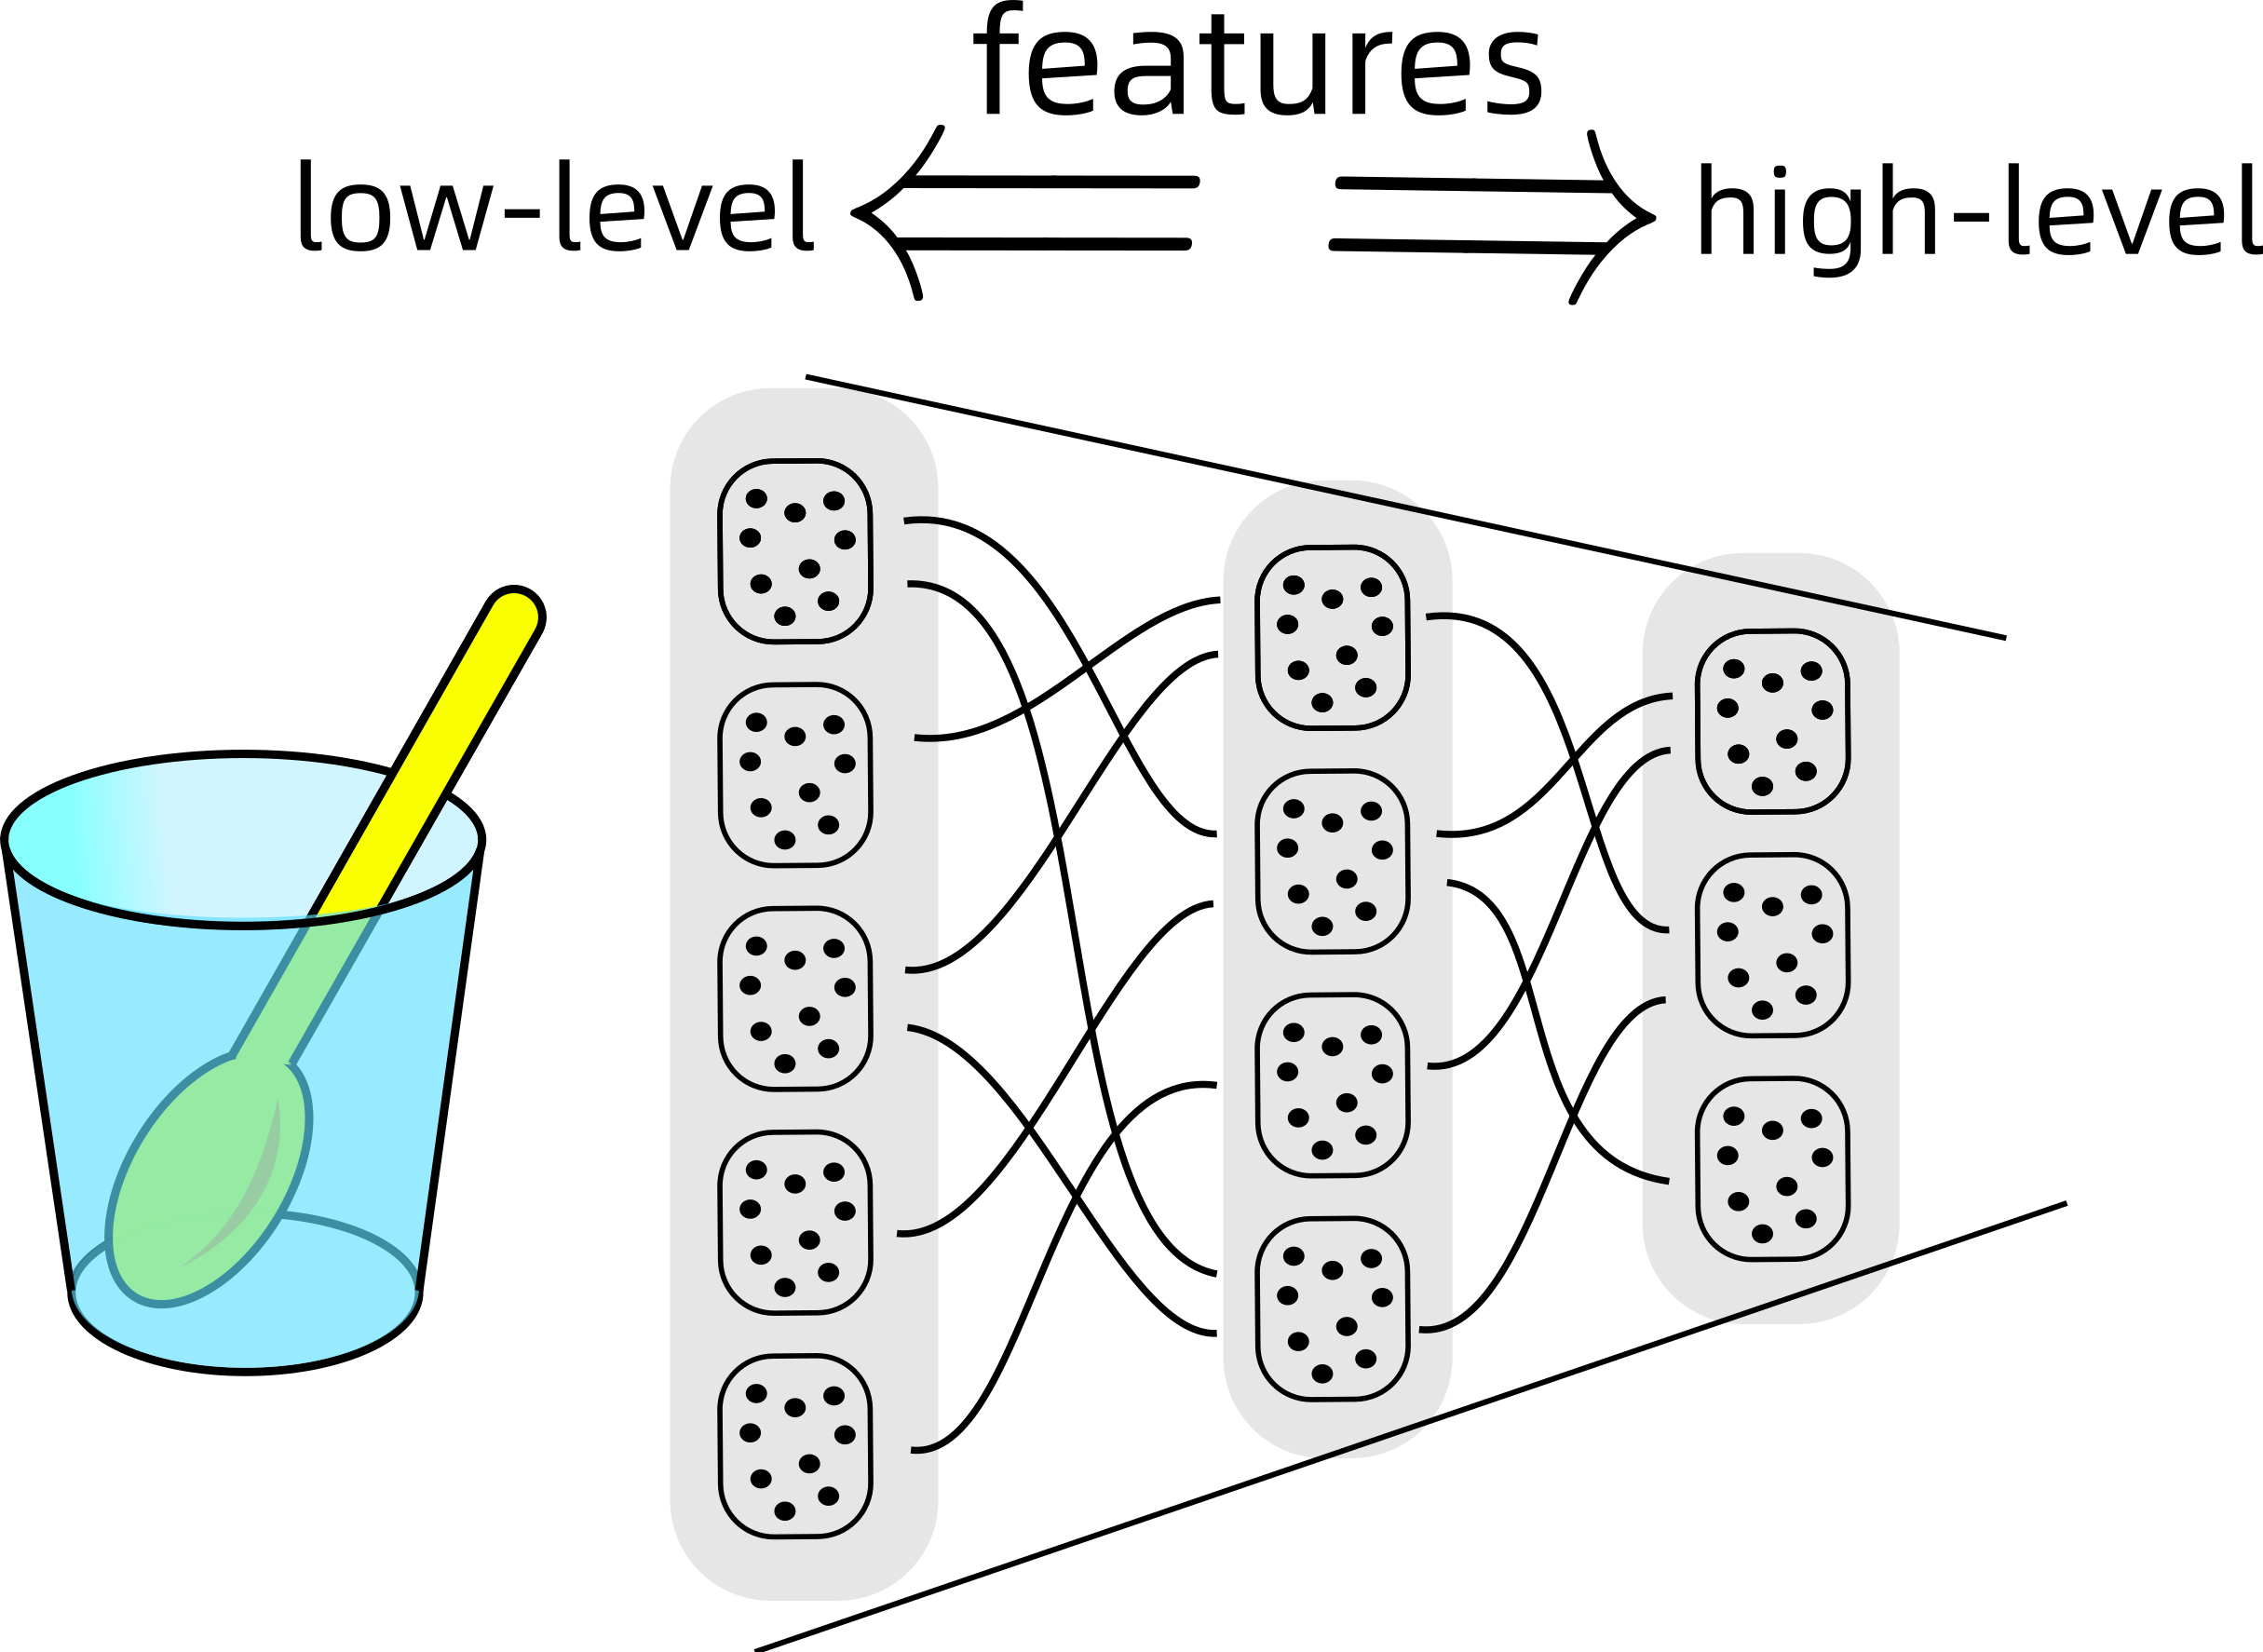
\includegraphics[scale=0.7]{hierarchical-features.png}}}
\end{equation}

Remember that in the Transformer, symbols are organized as \textbf{sequences}, for example: ``spoon $\cdot$ inside $\cdot$ glass.''  It may be desirable for AGI to have multiple levels of features, such as ``spoon'' and ``glass'' on a lower level, and ``inside'' on a higher level.

Juxtaposed side by side, the Transformer and the cortex seem to have many similarities:
\begin{equation}
\vcenter{\hbox{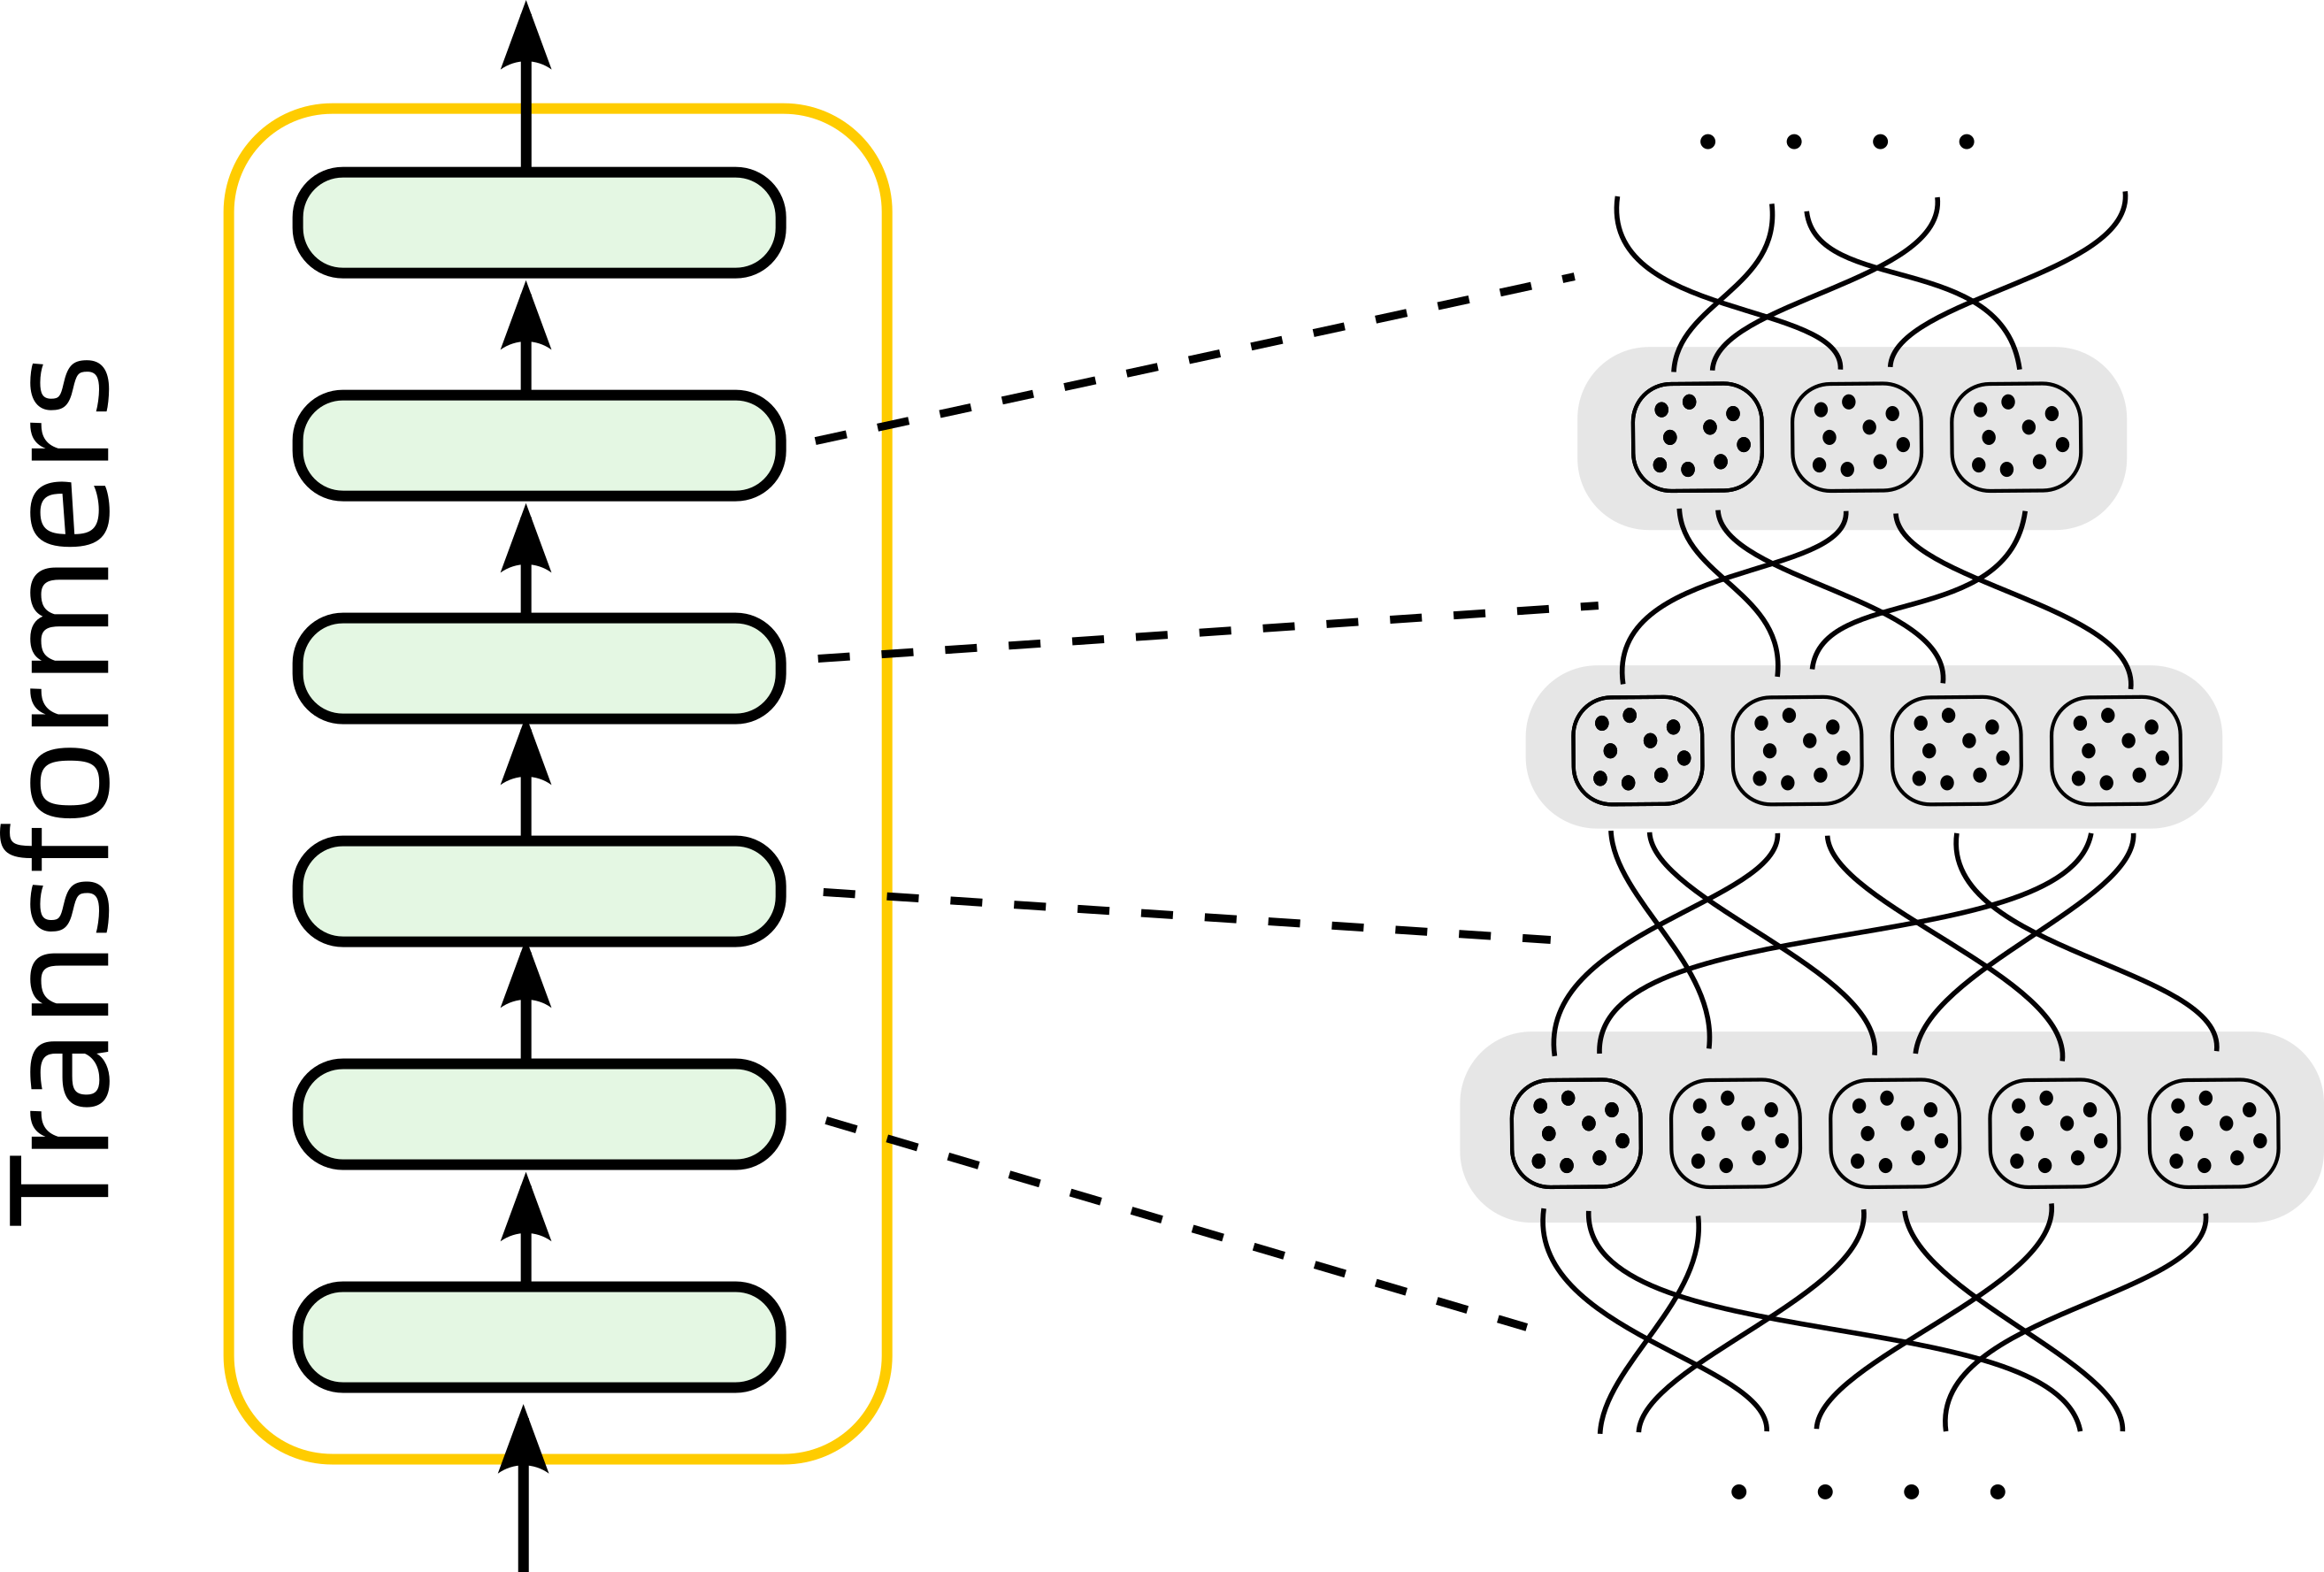
\includegraphics[scale=0.7]{Transformer-cortex-correspondence.png}}}
\end{equation}
Softmax corresponds to lateral inhibition.  The Transformer has many layers because it \textbf{unfolds} along the time axis the training of a recurrent network --- part of the reason why the Transformer is very efficient.  Each hidden layer of the Transformer can be construed as a ``stage'' of logical inference:
\begin{equation}
\mbox{input} \vdash \mbox{stage}_1 \vdash \mbox{stage}_2 \vdash .... \vdash \mbox{output}.
\end{equation}

Also recall that our reinforcement learning model consists of just the state and its transition function:
\begin{equation}
\vcenter{\hbox{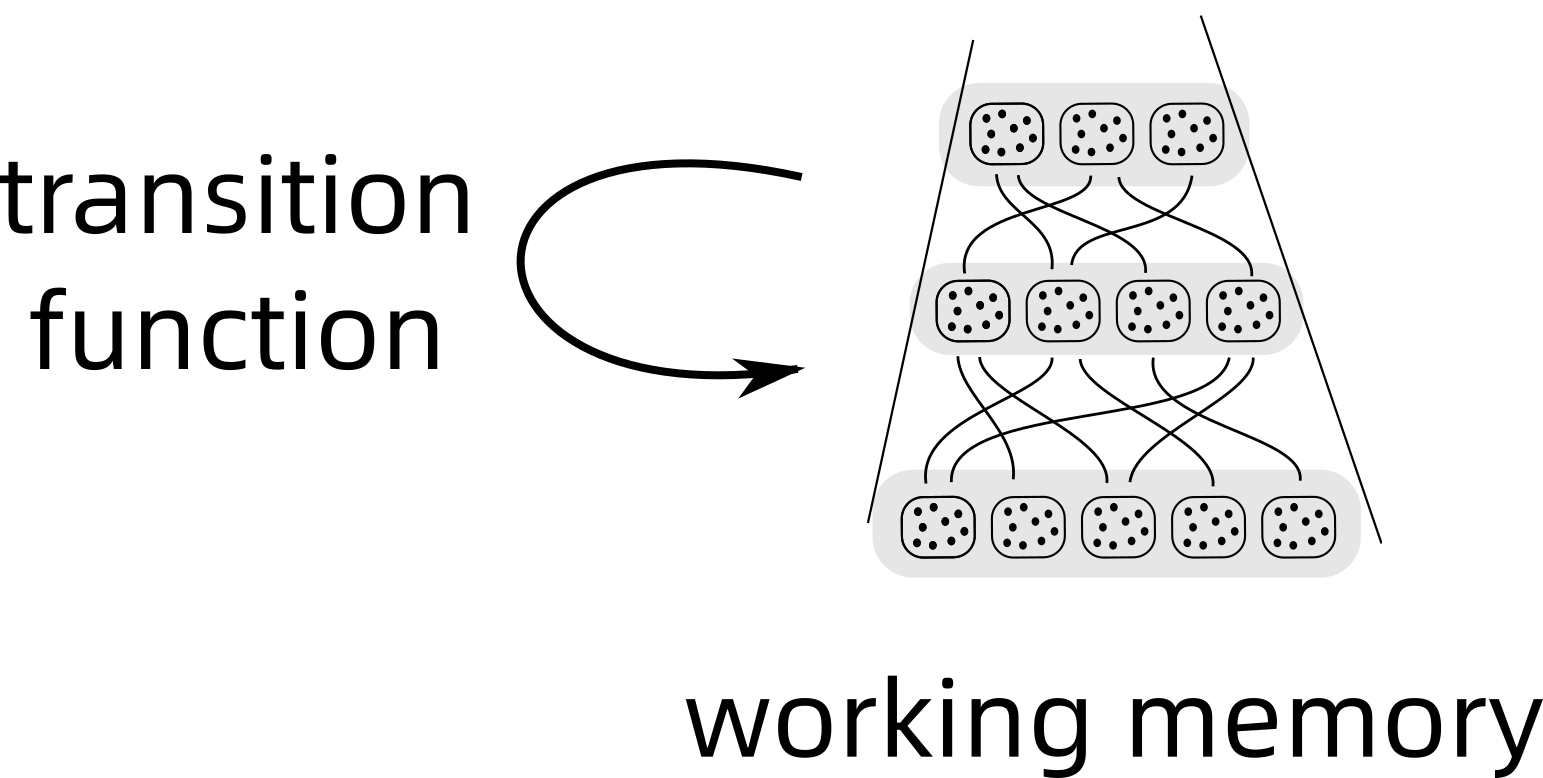
\includegraphics[scale=0.7]{cortex-with-transition-function.png}}}
\end{equation}
Based on this understanding, we need to figure out how to design the next version of Transformer and incorporate it into our AGI architecture....

\section{Abductive reasoning}
\label{sec:abductive-reasoning}

Abduction has been relatively neglected in AGI research, which had focused on forward inference.  Recently there is a call to study this important aspect.

In logic, abduction means finding the \textbf{explanation} for some known facts.  An explanation $E$ is simply some propositions that imply the known fact $F$, ie, $E \Rightarrow F$.

For example, why do we think a certain actress, say Marilyn Monroe, is ``sexy'' \footnote{I use this example because ``sexy'' is a kind of high-level concept and we apply this concept commonly when we meet other people.  Every one can relate to the ``reasons'' why we think someone is sexy.} ?  That's because we recognize she has some features (visual or otherwise, no need to enumerate them explicitly) that we consider sexy.  So, $E_1 \wedge E_2 \wedge .... \Rightarrow \mathrm{Sexy}$.  Those conditions \textbf{imply} she is sexy, and they are the \textbf{explanation} for her sexiness.

Why is abduction important?  For example, when a waitress says ``The Ham Sandwich left a big tip'', \textit{Ham Sandwich} here refers to the customer who ordered it (an example of metonymy).  The AI knows the plain facts such as that someone ordered a ham sandwich, and then it abduces that the most likely \textbf{interpretation} of the phrase ``Ham Sandwich'' is as the person associated with it.  This is the basis of \textbf{Abductive Interpretation of Natural Language} proposed by Jerry Hobbs:
\begin{equation}
\vcenter{\hbox{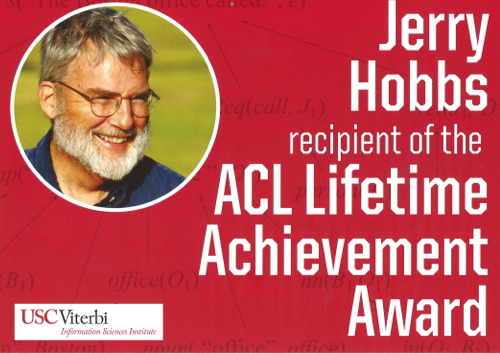
\includegraphics[scale=0.7]{Jerry-Hobbs.png}}}
\end{equation}

So abductive reasoning is basically just \textbf{bidirectional} inference.

When a system has both forward and backward connections, it forms a loop and its dynamics is likely to produce ``\textbf{resonance}''.  This harks back to the ART (\textbf{Adaptive Resonance Theory}) proposed by Grossberg and Carpenter beginning in the 1980s.

Such resonance behavior can be viewed as the system seeking to minimize an energy, ie, trying to find the ``best explanation'' to a set of facts.  

This is also corroberated by neuroscientific evidence:  areas in the cerebral cortex are replete with both forward- as well as \textbf{back-projections}, as depicted in diagram (\ref{fig:cortex-back-projections}).  We can further abstract this with the following diagram, where $F$ and $G$ are not functions but \textbf{optimization constraints}:
\begin{equation}
\begin{tikzcd}
\vec{y} \arrow[d, bend left, "G"]  \\
\vec{x} \arrow[u, bend left, "F"]
\end{tikzcd}
\end{equation}
If the input $\vec{x}$ produces the output $\vec{y}$ after some iterations, then it is likely that the output $\vec{y}$ would produce $\vec{x}$ in the \textbf{inverse} direction.  In other words, we have a \textbf{neural} mechanism that implements a function $f$ and its inverse $f^{-1}$.  The significance of this (from the \textbf{learning} point of view) is that we only need to learn the function $f$ and we get $f^{-1}$ \textbf{for free}.

In logic, if forward inference is denoted as $\vdash_{\KBsymbol}$, where $\KBsymbol$ is a set of logic rules, then abduction is $(\vdash_{\KBsymbol})^{-1}$.  Abductive interpretation is basically a \textbf{constraint-satisfaction} process that uses inference rules in both directions.

\section{Dealing with assumptions}

\end{preview}
\end{document}
